\section{Theorie}
\label{sec:theorie}

Bevor wir mit der Erläuterung des Faraday-Effekts beginnen, wiederholen wir zunächst einige Grundlagen der Festkörperphysik.

\subsection{Bandstruktur kristalliner Festkörper}

In kristallinen Festkörpern liegen die Gitteratome in einem periodischen Gitter.
Die dazugehörigen Elektronen sind dabei in der Lage, sich mehr oder weniger frei durch das Gitter zu bewegen.
Jedes Elektron jedes einzelnes Atoms besetzt dabei sein eigenes diskretes Energieniveau, sodass sich insgesamt eine überlappende Struktur
aus Energieniveaus bildet, die ein Band genannt wird.
So gibt es unterschiedliche Bänder, die meist nicht überlappen, sondern durch eine diskrete Bandlücke getrennt sind.
Hier sind insbesondere das Valenz- und das Leitungsband relevant.
Als Valenzband wird dabei das höchste auch bei $T=\SI{0}{\kelvin}$ besetzte Band bezeichnet; Leitungsband heißt dagegen das Band,
das bei Besetzung für die elektrische Leitfähigkeit des Festkörpers sorgt. \\

Je nachdem, wie groß die Bandlücke zwischen Valenz- und Leitungsband sind, lassen sich Festkörper in drei verschiedene Klassen einteilen.
Ist die Bandlücke so groß, dass sie auch bei thermischer Anregung nur schwer überwunden werden kann, sprich der Festkörper auch bei großen
Temperaturen nicht leitfähig wird, wird von einem Isolator gesprochen.
Die typische Bandlücke von Isolatoren liegt typischerweise im Bereich oberhalb von $\SI{3}{\eV}$.
Bei einer Bandlücke zwischen $\SI{1}{\eV}$ und $\SI{3}{\eV}$ wird der Festkörper als Halbleiter bezeichnet.
Hier ist es möglich, durch vergleichsweise geringe thermische Anregung eine deutliche Steigerung der Leitfähigkeit möglich.
Metalle dagegen besitzen keinerlei Bandlücke; das Valenzband und das Leitungsband überlappen sich zumindest teilweise, sodass auch ohne
thermische Anregung Strom fließt. \\

Hier interessieren uns insbesondere Halbleiter, insbesondere dotierte Halbleiter.
Der Prozess der Dotierung, also der Einführung von Fremdatomen in ein Material, wird bei Halbleitern genutzt, um die Eigenschaften der
elektrischen Leitfähigkeit zu verändern.
Dabei unterscheiden wir p- und n-Dotierung.
Die p-Dotierung beschreibt dabei die Einführung sogenannter Akzeptoren, also Fremdatomen,
die weniger Elektronen als das ersetzte Ursprungsatom besitzt und so zu einem Loch innerhalb des Valenzbandes.

Bei der n-Dotierung werden dagegen Donatoren, also Atome mit Überschusselektronen in den Halbleiter eingeführt.
Die Fremdatome bei der  n-Dotierung sind dabei so gewählt, dass ihr Energieniveau knapp unter dem des Leitungsbands,
aber deutlich über dem des Valenzbandes liegt.
So erhöht die n-Dotierung die elektrische Leitfähigkeit des Festkörpers.


\subsection{Effektive Masse}

Das Konzept der effektiven Masse, hier von den Elektronen im Festkörper, beschreibt die Ersetzung der Masse $m$ durch eine veränderte Masse

\begin{equation}
    m^*_i = \frac{\hbar^2}{\left[\frac{\partial^2 E}{\partial k^2_i} \right]_{k_i=0}} \,,
    \label{eq:effektivemasse}
\end{equation}
wobei $i = x,y,z$ mit den Komponenten $k_i$ des Wellenvektors der Elektronen.
Diese effektive Masse $m^*$ folgt aus einer Taylorentwicklung der Energie $E(\vec{k})$ bis zur zweiten Ordnung um $k=0$ und berücksichtigt das Gitterpotential,
die bei der quasifreien Bewegung der Elektronen durch das Gitter mit ihnen wechselwirken.
Da bei den hier verwendeten GaAs-Proben eine hinreichend hohe Gittersymmetrie gegeben ist, ist die effektive Masse nicht richtungsabhängig.


\section{Zirkulare Doppelbrechung}

Die zirkulare Doppelbrechung beschreibt, wie in \autoref{fig:doppelbrechung} schematisch dargestellt,
die Drehung der Polarisationsebene linear polarisierten Lichts beim Einfall in ein Kristallmedium.

\begin{figure}[H]
    \centering
    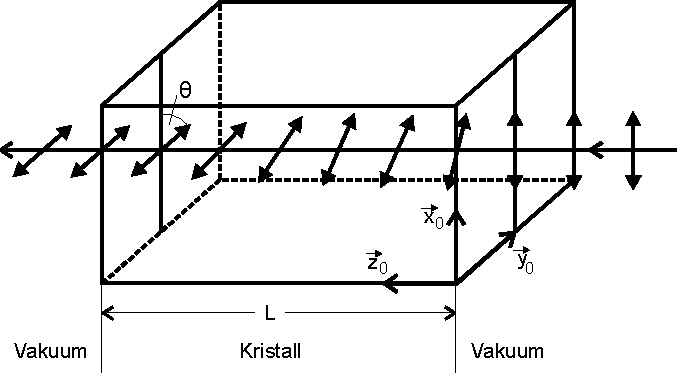
\includegraphics[width=.6\textwidth]{figures/doppelbrechung.pdf}
    \caption{Schematische Darstellung der Drehung der Polarisationsebene einfallenden linear polarisierten Lichts in einem kristallinen Medium um den Winkel $\theta$ \cite{doppbre}.}
    \label{fig:doppelbrechung}
\end{figure}

Um den Effekt anschaulich zu erklären, sei angenommen, dass linear polarisiertes Licht aus einer Überlagerung zweier zirkular polarisierten
entgegengesetzter Umlaufrichtungen besteht.

Ist in dem betrachteten Medium die Phasengeschwindigkeit links und rechts polarisierter Wellen unterschiedlich, verschiebt sich das Gleichgewicht zwischen
den beiden zirkular polarisierten Wellen, sodass effektiv eine Drehung der Polarisationsebene zu beobachten ist.
Ein solches Medium wird auch als aktives Medium bezeichnet. \\

Die Diskrepanz in den Phasengeschwindigkeiten zwischen Licht unterschiedlicher Polarisationsrichtungen lässt sich auf im Medium induzierte Dipole zurückführen.
Konkret entstehen diese induzierten Dipole durch elektrische Dipolmomente der Gitteratome und durch die Wechselwirkung der Bandelektronen mit den Atomrümpfen.

Insgesamt entsteht so eine makroskopische Polarisation
\begin{equation}
    \vec{P} = \varepsilon_0 \chi \vec{E}
    \label{eq:polarisation} 
\end{equation}
mit der Influenzkonstante $\varepsilon$ für hinreichend geringe E-Felder $\vec{E}$.
Die dielektrische Suszeptibilität $\chi$ ist in doppelbrechenden Medien ein Tensor mit nicht-diagonalen komplex-konjugierten Koeffizienten der Form
\begin{equation*}
    \chi = \left( \begin{matrix}
        \chi_{xx}     & i\chi_{xy}    & 0 \\
        - i \chi_{xy} & \chi_{yy}     & 0 \\
        0             & 0             & \chi_{zz}
    \end{matrix}\right) \,,
\end{equation*}
sodass sich der Rotationswinkel 
\begin{align*}
    \theta &= \frac{L}{2} (k_R - k_L) \\
           &= \frac{L \omega}{2} \left(\frac{1}{v_{\text{ph},R}} - \frac{1}{v_{\text{ph},L}}\right) \\
           &= \frac{L \omega}{2 c} (n_R - n_L)
\end{align*}
mit der Phasengeschwindigkeit $v_{L/R} = \frac{1}{k_{L/R}}$ und dem Brechungsindex $n_{L/R} = \frac{c}{v_{L/R}}$ in guter Näherung zu
\begin{equation}
    \theta = \frac{L \omega}{2 c n} \chi_{xy}
    \label{eq:thetanoB}
\end{equation}
ergibt.

\section{Faraday-Effekt}

Während die bisher diskutierte zirkulare Doppelbrechung nur bei optisch aktiver Materie auftritt, diskutieren wir jetzt den Spezialfall, 
bei dem es unter Anlegung eines äußeren Magnetfelds parallel zur Einfallsebene des Lichts auch bei optisch inaktiver Materie zur zirkularen Doppelbrechung kommt.
Hier wird dann explizit vom Faraday-Effekt gesprochen.

So lässt sich aus der Bewegungsgleichung für gebundene Elektronen eine Verschiebungspolarisation von $\vec{P} = - N e_0 \vec{r}$ herleiten.
Dabei ist $N$ die Anzahl der Elektronen pro Volumeneinheit und $e_0$ die Elementarladung.
Nach einiger Rechnung folgt näherungsweise
\begin{equation*}
    \theta = \frac{2 \pi^2 e^3_0 c}{\varepsilon_0 m^2} \frac{1}{ \lambda^2 \omega_0^4} \frac{N B L}{n}
\end{equation*}
für den Rotationswinkel $\theta$ bei Durchqueren des Mediums der Dicke $L$ und anliegender Magnetfeldstärke $B$ für Licht der Wellenlänge $\lambda$.
Die Resonanzfrequenz der Elektronen wird dabei durch $\omega_0$ beschrieben. \\

Im Limes $\omega_0 \rightarrow 0$ finden wir mit der effektiven Masse der Elektronen $m^*$

\begin{equation}
    \theta_\text{frei} = \frac{e^3_0}{8 \pi^2 \varepsilon_0 c^3} \frac{1}{(m^*)^2} \lambda^2 \frac{N B}{n}
\end{equation}
für $\theta_\text{frei} = \frac{\theta}{L}$.
Dabei sind die Einheiten so gewählt, das die effektive Masse $m^*$ in $\si{\kilo\gram}$ angegeben ist.
So lässt sich aus bekannten und messbaren Parametern die effektive Masse der Elektronen bestimmen.


